\subsection{Position Specific Score Matrix}

\acrfull{pssm} is a very useful protein feature. The protein feature represented by PSSM depends on the sequence of all the proteins in consideration. The HUMAN genome protein (a database of more than 100,000) is downloaded from UniProt Library and we construct the PSSM matrix for each of the kinase proteins based on this HUMAN Genome Protein Database. Doing so, we try to characterize the PSSM matrix according to human proteins in a motivation to anticipate the prediction of new identified kinase proteins.

\begin{table}
  \centering
  \caption{PSSM Analysis Design} 
  \begin{subtable}[]{protein fasta sequence}
    \begin{tabular}{|l|l|}
    \hline
    
    1 & GAGGTAAAC \\ \hline
    2 & TCCGTAAGT \\ \hline
    3 & CAGGTTGGA \\ \hline
    4 & ACAGTCAGT \\ \hline
    5 & TAGGTCATT \\ \hline
    6 & TAGGTACTG \\ \hline
    7 & ATGGTAACT \\ \hline
    8 & CAGGTATAC \\ \hline
    9 & TGTGTGAGT \\ \hline
    10 & AAGGTAAGT \\ \hline
    
    \end{tabular}
    
  \end{subtable}

  \begin{subtable}[]{Frequency Table}
    \begin{tabular}{|l|l|l|l|l|l|l|l|l|l|}
    \hline
    
     & 1 & 2 & 3 & 4 & 5 & 6 & 7 & 8 & 9 \\ \hline
    A & 3 & 6 & 1 & 0 & 0 & 6 & 7 & 2 & 1 \\ \hline
    C & 2 & 2 & 1 & 0 & 0 & 2 & 1 & 1 & 2 \\ \hline
    G & 1 & 1 & 7 & 10 & 0 & 1 & 1 & 5 & 1 \\ \hline
    T & 4 & 1 & 1 & 0 & 10 & 1 & 1 & 2 & 6 \\ \hline
    
    \end{tabular}
  \end{subtable}

  \begin{subtable}[]
    {Log-Likelihood Matrix}
    \begin{tabular}{|l|l|l|l|l|l|l|l|l|l|}
    \hline 

        & 1 & 2 & 3 & 4 & 5 & 6 & 7 & 8 & 9 \\ \hline
    A & 0.3 & 0.6 & 0.1 & 0.00 & 0.00 & 0.6 & 0.7 & 0.2 & 0.1 \\ \hline
    C & 0.2 & 0.2 & 0.1 & 0.00 & 0.00 & 0.2 & 0.1 & 0.1 & 0.2 \\ \hline
    G & 0.1 & 0.1 & 0.7 & 1.00 & 0.00 & 0.1 & 0.1 & 0.5 & 0.1 \\ \hline
    T & 0.4 & 0.1 & 0.1 & 0.00 & 1.00 & 0.1 & 0.1 & 0.2 & 0.6 \\ \hline
    
    \end{tabular}
  \end{subtable}

  \begin{subtable}[]
    {Log-Likelihood Matrix for the motif}
    \begin{tabular}{|l|l|l|l|l|l|l|l|l|l|}
    \hline 
    
        & 1 & 2 & 3 & 4 & 5 & 6 & 7 & 8 & 9 \\ \hline
    A & 0.3 &  &  &  &  &  & 0.7 &  &  \\ \hline
    C &  &  & 0.1 & 0.00 & 0.00 & 0.20 &  &  & 0.2 \\ \hline
    G &  & 0.1 &  &  &  &  &  & 0.5 &  \\ \hline
    T &  &  &  &  &  &  &  &  &  \\ \hline
    
    \end{tabular}
    \caption{Sliding Window Score Calculation}
    \label{table:motif_movement}
  \end{subtable}
  
  \label{table:PSSM_Analysis} 
\end{table}

The Table \ref{table:PSSM_Analysis} shows a rudimentary process of calculating PSSM score values. The sequence following shows the process of calculating the scores once the PSSM distribution of the whole family is calculated. Table \ref{table:motif_movement} shows the score distribution of lowercase amino acid sequence (starting after 4th position) determined by the size of the sliding window.

\seqsplit{ACTC\textbf{agccccagc}GGAGGTGAAGGACGTCCTTCCCCAGGAGCCGGTGAGAAGCGCAGTCGGGGGCACGGGGATGAGCTCAGGGGCCTCTAGAAAGATGTAGCTGGGACCTCGGGAAGCCCTGGCCTCCAGGTAGTCTCAGGAGAGCTACTCAGGGTCGGGCTTGGGGAGAGGAGGAGCGGGGGTGAGGCCAGCAGCA} 

\begin{wraptable}{br}{5.5cm}
% \begin{table}[!ht]
    \centering
    \caption{Score of sliding window motifs} \label{wrapTable:pssm-score}
    \begin{tabular}{|l|l|}
    \hline
    
    0 & 1.099 \\ \hline
    1 & 1 \\ \hline
    2 & 2.2 \\ \hline
    3 & 2.1 \\ \hline
    4 & 2.1 \\ \hline
    5 & 1.300 \\ \hline
    6 & 1.3 \\ \hline
    7 & 1.4 \\ \hline
    8 & 2 \\ \hline
    9 & 2.9 \\ \hline
    
    \end{tabular}
% \end{table}
\end{wraptable}

.3, .1, .1, 0, 0, .2, .7, .5, .2  == Sum(2.1) - posix(4) -- See Table \ref{wrapTable:pssm-score}

\begin{figure}
    \centering 
          %  \subfloat[]{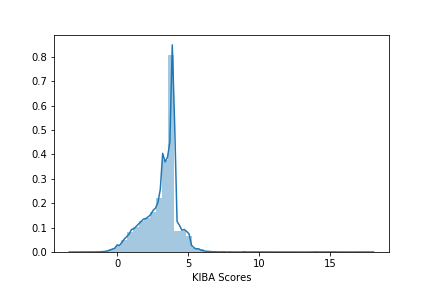
\includegraphics[width=.3\textwidth]{mainmatter/3-Methodology/images/data/distribution.png}}
           \subfigure[KIBA Scores]{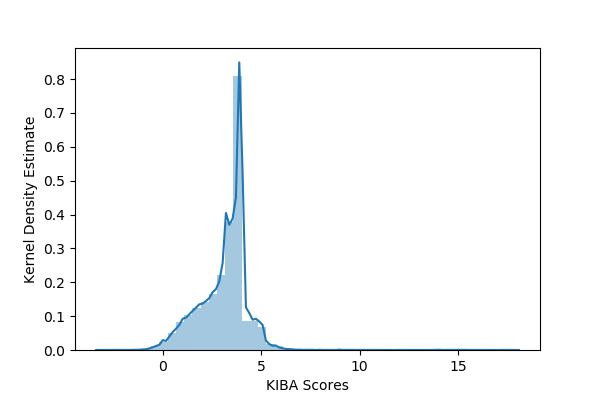
\includegraphics[width=.7\textwidth]{mainmatter/3-Methodology/images/figures/distribution.png}}
           \subfigure[Logarithmic One Hot Encodings of Drug Sequence]{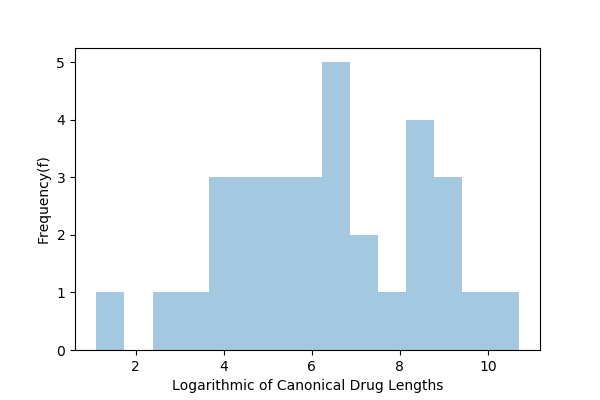
\includegraphics[width=.7\textwidth]{mainmatter/3-Methodology/images/figures/drug_length_logarithmic.png}}
           \subfigure[One Hot Encodings of Protein Sequence]{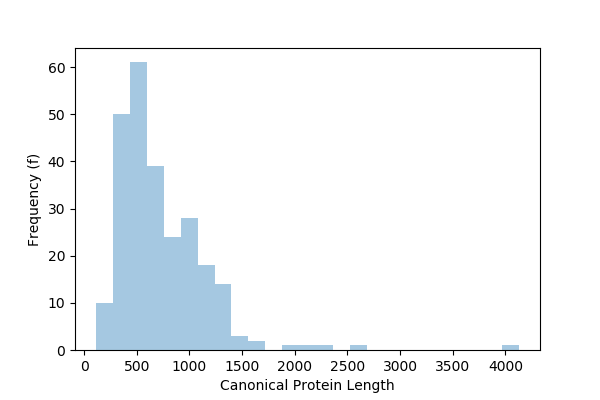
\includegraphics[width=.7\textwidth]{mainmatter/3-Methodology/images/figures/prot_length.png}}
           \caption[Dataset Distribution]{Data Distribution of KIBA-interaction scores, Drug Sequences and Protein Sequences}
           \label{fig:kiba_drug_protein}
\end{figure}
  
\iffalse
  \subsection{UniProt and CHEMBL}
  
  \subsubsection{UniProt} 
  The sequence related information of protein is referenced using UniProt Identifier and protein sequence (FASTA) is called using the api from UniProt. \cite{UniProtConsortium2018}
  
  
  \subsubsection{CHEMBL}
  The molecular fingerprints related to drugs are referenced usning CHEMBL Identifier and the drug sequence is called from CHEMBL database. \cite{Gaulton2017}
  \fi
  \subsection{PSI-BLAST}
  PSI-Blast tools relates with multiple sequence alignments from a family of protein sequences\cite{Schaffer2001}. This helps us to create a \acrshort{pssm} - Equation (\ref{eq:pssm}) - matrix referred to as secondary protein structure. The improvement in drug-contact prediction can be thought for amino acid composition being tuned with the scoring system. For this study, the PSSM profile of every protein sequence is obtained by executing iteration of PSI-BLAST against \cite[KEGG]{Schaffer2001} protein. PSSM profile is a matrix of L*20 dimensions where, 20 referring to standard type of amino acids and L being the length of the protein. The larger positive scores represent conserved positions, which in turn implies critical functional residues that are required to perform various intermolecular interactions.\cite[PSSM]{Schaffer2001}
  
  \begin{equation}
    PSSM = \begin{bmatrix}
      P_{1,1} & P_{1,2} & \dots & P_{1,20} \\
      P_{2,1} & P_{2,2} & \dots & P_{2,20} \\
      \vdots  & \vdots  & \ddots & \vdots \\
      P_{2,1} & P_{2,2} & \dots & P_{2,20} \\
    \end{bmatrix}
    \label{eq:pssm}
  \end{equation}
  
  \subsubsection{PSSM-DT}
  Two forms of \acrshort{pssm} distance transformation techniques are used to transform the \acrshort{pssm} information into fixed dimensional vectors \cite{Xu2015}. The PSSM-DT (PSSM-Distance Transformation) can transform the \acrshort{pssm} information into uniform numeric representation by approximately measuring the occurrence probabilities of any pairs of amino acid. It results in two types of feature matrices: PSSM-SDT and PSSM-DDT defined by:
  
  \begin{equation}
    PSSM-SDT(i,lg) = \sum_{i=1}^{L-lg} S_{i,j} \times \frac{ S_{i,j+lg} }{L-lg} 
    \label{eq:pssmsdt}
  \end{equation}
  \textit{\center lg =  distance of separation between same amino acid sequence}
  
  \begin{equation}
    PSSM-DDT(i_1,i_2, lg) = \sum_{j=1}^{L-lg} S_{i_1,j} \times \frac{ S_{i_2,j+lg} }{ L-lg} 
    \label{eq:pssmddt}
  \end{equation}
  \textit{\centering i\textsubscript{1} and i\textsubscript{2} refer to tow different types of amino acids}
  
  Thus we have [380 ~\eqref{eq:pssmddt}+20 ~\eqref{eq:pssmsdt} = 400] x lg matrix which will be used as protein-specific vector in this work.
  
  \subsubsection{Evolutionary Distance Transformation Matrix}
  The mutational information of protein can be more informative than the sequence information itself\cite{Zhang2014}. Evolutionary difference formula(EDF) is used to represent mutation difference between adjacent residues. Secondly, the PSSM is converted into 20 x 20 matrix (ED-PSSM). This extracts the non co-occurrence probability for two amino acids separated by a certain distance \textit{d} in the protein from the PSSM profile. For example, d=1 implies that the two amino acids are consecutive; d=2 implies that there is one amino acid between the two. Then the EDT feature vector computed from ED-PSSM can be represented as (~\ref{eq:Pmat}): 
  \begin{equation}
    \label{eq:Pmat}
    P = [ \partial_1 ,\partial_2, \dots, \partial_\Omega]
  \end{equation}
  where $\Omega$ is an integer that represents the dimension of the vector whose value is 400.. The non-co-occurrence probability of two amino acids separated by distance \textit{d} can be computed as:
  \begin{equation}
    f(A_x,A_y) = \sum_{d=1}^{D} \frac{1}{L-d} \sum_{i=1}^{L-d} (P_{i,x} - P_{i+d,y})^2
    \label{eq:edt}
  \end{equation}
  where $P_{i,x}$ and $P_{i+d,y}$ are the elements in the PSSM profile; $A_x$ and $A_y$ represent any of the the 20 different amino acids in the protein sequence. Finally we spread the $f(A_x,A_y)$ in equation ~\ref{eq:Pmat} as:
  $ \partial_1 = f(A_1,A_2) $, 
  $ \partial_{400} = f(A_{20}, A_{20}) $
  
  
  \subsection{Residue feature} 
  The Statistical Residue Vector Space \acrshort{srv} \cite{Wong2018} plays an important role in Residue Residue Interaction and thus creates a basis for structural stability of the protein sequence itself. Though related more to the tertiary structure of protein sequence itself, we regard it to create a correlated sequence information where two proteins are related distantly by sequence but highly related with functional characteristic of protein. Table ~\ref{table:r2r} shows the table used in this work. It is a 20 x 20 matrix whose rows and columns represent 20 standard amino acids.
  
  \subsubsection{Residue Probing Transformation(RPT) feature}
  RPT as proposed by Jeong et al.\cite{Jeong2011}, and implemented by Pujan et al.\cite{Mishra2019}, emphasize domains with similar conservation rates by grouping domain families based on their conservation score in the PSSM profile.
  \begin{equation}
    RPT = \begin{bmatrix}
      S_{1,1} & S_{1,2} & \dots & S_{1,20} \\
      S_{2,1} & S_{2,2} & \dots & S_{2,20} \\
      \vdots  & \vdots  & \ddots & \vdots \\
      S_{2,1} & S_{2,2} & \dots & S_{2,20} \\
    \end{bmatrix}
    \label{eq:rpt}
  \end{equation}
  The RPT matrix (Equation ~\ref{eq:rpt}) is then tranformed into feature vector of 400 dimensions, as shown in Equation ~\ref{eq:rptV}.
  
  \begin{equation}
    V = [ f_{s_{1,1}}, f_{s_{1,2}}, \dots, f_{s_{i,j}}, \dots, f_{s_{20,20}} ]
    \label{eq:rptV}
  \end{equation}
  where, 
  \begin{equation}
    f_{s_{i,j}} = \frac{s_{i,j}}{L} (i,j = 1,2,\dots,20)
    \label{eq:rptF}
  \end{equation}

  \subsection{Labelled Encodings}
  
  The labeled encoding techniques is used to represent the canonical structure of drugs and proteins. The structural canonical information is preserved while sending the feature set to deep learning method. An array of integers is formed from particular sequence while representing the structural information.
  
  The Labelled Encodings of protein and drugs can be defined by Table \ref{table:label_encoding} :
  \begin{table}[h]
    \centering
    \begin{subtable}{Protein Labeled Encoding Technique}
      \centering
      % \caption{Protein Labeled Encoding Technique}
      \begin{tabular}{|cccc|}
        \hline
        A --> 1 & C --> 2 & B --> 3 & E --> 4 \\ \hline
        D --> 5 & G --> 6 & F --> 7 & I --> 8 \\ \hline
      \end{tabular}
    \end{subtable}  

    \begin{subtable}{Drugs Labeled Encoding Technique}
      \centering
      % \caption{Drugs Labeled Encoding Technique}
      \begin{tabular}{|cccc|}
        \hline
        \# --> 1 & \% --> 2 & : --> 3 & + --> 5 \\ \hline
        4 --> 13 & 7 --> 14 & F --> 25 & I --> 26 \\ \hline
      \end{tabular}
    \end{subtable}
    \caption{Labeled Encoding of Proteins and Drugs}
    \label{table:label_encoding}
  \end{table}
  
  % CHARPROTSET = { "A": 1, "C": 2, "B": 3, "E": 4, "D": 5, "G": 6,
	% 			"F": 7, "I": 8, "H": 9, "K": 10, "M": 11, "L": 12,
	% 			"O": 13, "N": 14, "Q": 15, "P": 16, "S": 17, "R": 18,
	% 			"U": 19, "T": 20, "W": 21,
	% 			"V": 22, "Y": 23, "X": 24,
	% 			"Z": 25 }

  % CHARCANSMISET = { "#": 1, "%": 2, ")": 3, "(": 4, "+": 5, "-": 6,
	% 		 ".": 7, "1": 8, "0": 9, "3": 10, "2": 11, "5": 12,
	% 		 "4": 13, "7": 14, "6": 15, "9": 16, "8": 17, "=": 18,
	% 		 "A": 19, "C": 20, "B": 21, "E": 22, "D": 23, "G": 24,
	% 		 "F": 25, "I": 26, "H": 27, "K": 28, "M": 29, "L": 30,
	% 		 "O": 31, "N": 32, "P": 33, "S": 34, "R": 35, "U": 36,
	% 		 "T": 37, "W": 38, "V": 39, "Y": 40, "[": 41, "Z": 42,
	% 		 "]": 43, "_": 44, "a": 45, "c": 46, "b": 47, "e": 48,
	% 		 "d": 49, "g": 50, "f": 51, "i": 52, "h": 53, "m": 54,
	% 		 "l": 55, "o": 56, "n": 57, "s": 58, "r": 59, "u": 60,
	% 		 "t": 61, "y": 62 }
  
  \section{Deep Learning Model}
  
  The Features thus formed are then subjected to deep learning model using keras library in python. We use the Embedding feature provided by keras as other features for both drug fingerprint and protein sequence. The implemented model is represented by Figure ~\ref{fig:dlm}. The input layers are described in Table ~\ref{table:inputs}.
  
  \begin{figure}[ht]
  \centering
  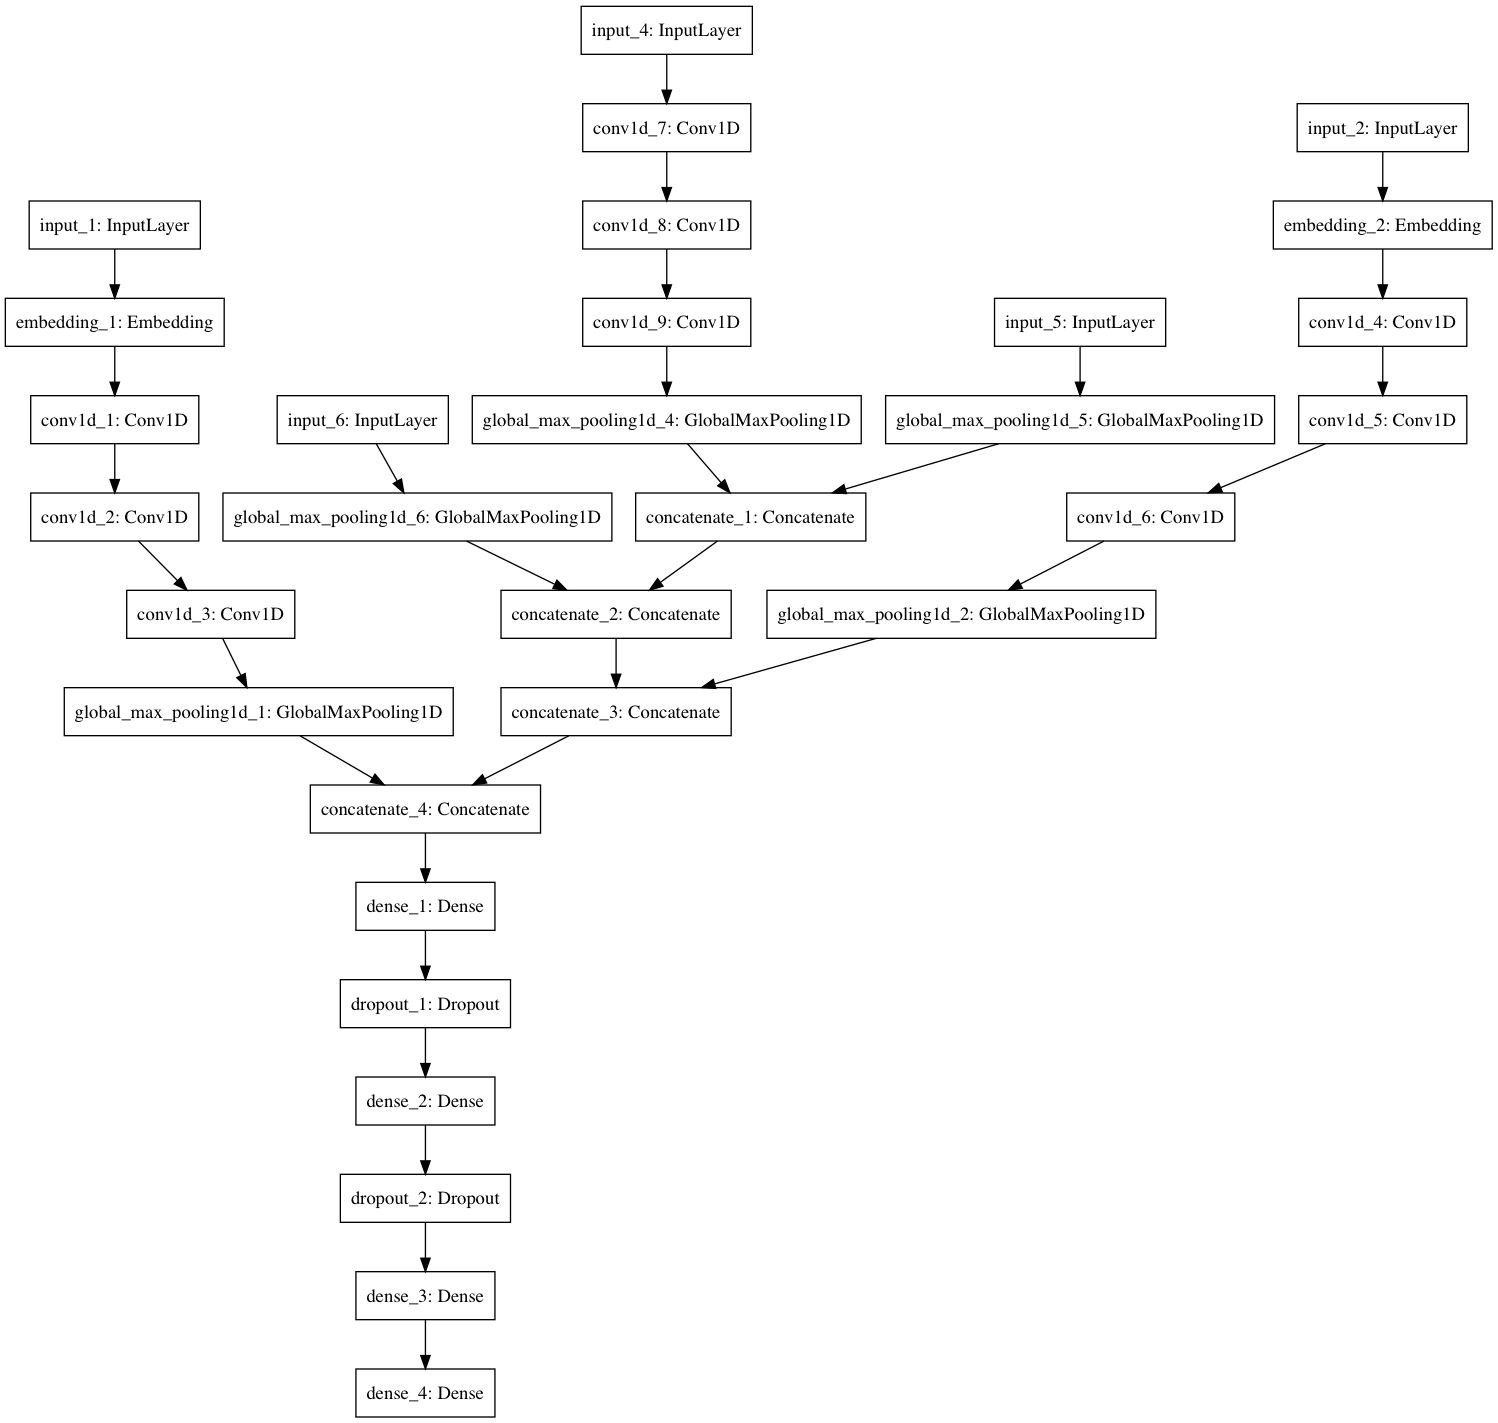
\includegraphics[width=1\linewidth]{mainmatter/3-Methodology/images/build_combined_categorical_tensor_contact_new.png}
  \caption{Deep Learning Model to predict Protein-Drug Interaction}
  \label{fig:dlm}
  \end{figure}
  \begin{table}[ht]\centering
    \caption{Inputs Used in the Deep Learning Network} 
    \begin{tabular}{|l|l|l|l|}
      \hline 
      S.No. & Input Layer Name & Used Feature Vector & Type \\ \hline
      1 & input\_1 & Label Encodings & Drug \\ \hline
      2 & input\_2 & Label Encodings & Protein \\ \hline
      3 & input\_3 & Evolutionary Distance Transformation Vector& Protein \\ \hline
      4 & input\_4 & PSSM-DT Vector & Protein \\ \hline
      5 & input\_5 & Residue Probing Transformation Vector & Protein \\   \hline 
    \end{tabular} 
    \label{table:inputs}
  \end{table}
  
  \subsection{Components description used from Tensorflow (Keras)}
  \subsubsection{Embedding Layer}
  The one-hot encodings of the drugs and protein sequences are inputs to this layer. It turns positive integers (indexes) into dense vectors of fixed size. eg. [[4], [20]] -> [[0.25, 0.1], [0.6, -0.2]].
  
  \subsubsection{Dense Layer}
  Dense Layer is a neural layer which fully connects the input layer to output layer. It can be used to learn the global pattern of the feature data. The representation can be seen from Figure ~\ref{fig:dense}.
  \begin{figure}[ht]
    \centering
    % 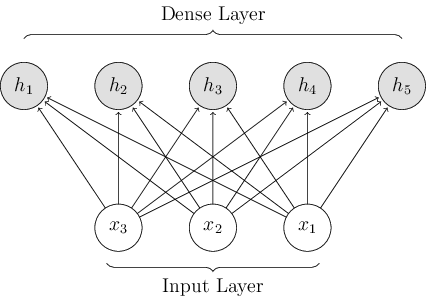
\includegraphics[width=.5\linewidth]{mainmatter/3-Methodology/images/dense.png}
    
  

\begin{tikzpicture}[->,>=stealth',shorten >=1pt,auto,node distance=2.8cm,
    semithick]

      \tikzstyle{every state}=[text=black]
      \node[state]          (A)   {$h_1$};
      \node[state]         (B)  [right of=A] {$h_2$};
      \node[label=above:{Dense Layer},state]         (C) [right of=B] {$h_3$} ;
      \node[state]         (D) [right of=C] {$h_4$};
      \node[state]         (E) [right of=D] {$h_5$};

      \node[state]         (X1) [below of=B] {$x_3$};
      \node[state, label=below:{Input Layer}]         (X2) [right of=X1]       {$x_2$};
      \node[state]         (X3) [right of=X2]       {$x_1$};

      \path (X1) 
      edge              node {} (A)
      edge              node {} (B)
      edge              node {} (C)
      edge              node {} (D)
      edge              node {} (E)
      % edge              node {1,1,R} (C)
      (X2) 
      edge              node {} (A)
      edge              node {} (B)
      edge              node {} (C)
      edge              node {} (D)
      edge              node {} (E)
      % edge              node {0,1,L} (C)
      (X3)
      edge              node {} (A)
      edge              node {} (B)
      edge              node {} (C)
      edge              node {} (D)
      edge              node {} (E);
      % edge [bend left]  node {1,0,R} (E);

\end{tikzpicture}

  
\caption{Dense Layer}
\label{fig:dense}
\end{figure}

  
  \subsubsection{Dropout Layer}
  Our model becomes undesirable when every component of the input layer makes a significant changes to the output layer. To reduce the effect of unimportant features we use dropout layer. Thus the backpropagation network tries to ignore the noise features and minimizes the unrealizable prediction of the learning problem. This can be expressed diagrammatically in the Figure ~\ref{fig:dropout}.
  \begin{figure}
    [ht] \centering
    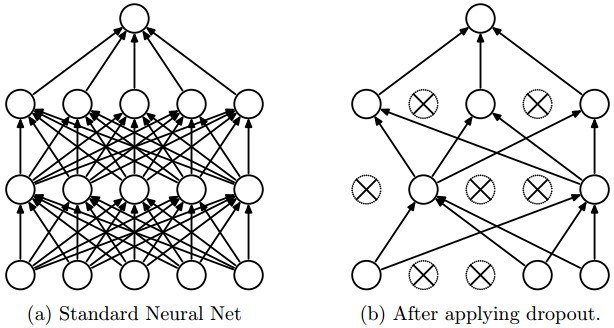
\includegraphics[width=.5\linewidth]{mainmatter/3-Methodology/images/dropout.jpeg}
    \caption[Dropout Layer]{a) Standard neural network whose all the nodes have weights connected to higher nodes and lower nodes. b) Certain nodes belonging to same levels are disconnected. Some weights are also disconnected from other nodes depending on the percentage of dropout applied.}
    \label{fig:dropout}
  
  \end{figure}
  
  \subsubsection{Pooling Layer}
  The Pooling layer is used to downsample the learned parameters from the grid of 3 dimensions returned by Convolution Layer. It gets reduced to 1 dimension by taking the highest values from the window size(corresponding to shape of 1\textsuperscript{st} dimensional element).
  \begin{figure}
    [ht]\centering
    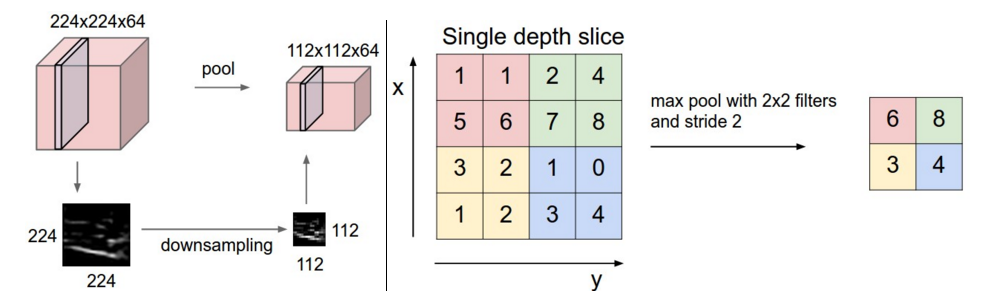
\includegraphics[width=.75\linewidth]{mainmatter/3-Methodology/images/pooling.png}
    \caption{Pooling Layer}
    \label{fig:pool_layer}
  \end{figure}
  
  \subsubsection{Concatenation Layer}
  Concatenation Layer as the name implies is used to simply join two vectors so that we create a feature set comprising of multiple features whose positional index indicates the feature set being manipulated.
  
  \subsubsection{Convolution Neural Network}
  To learn the local patterns in the input vector, we use \acrshort{cnn}. While Dense Layers and \acrshort{lstm} learn the global patterns, \acrshort{cnn} is used to understand the local patterns. It does so by increasing the depth layer, which in turn is designed to learn different patterns as shown in Figure ~\ref{fig:cnn}.
  \begin{figure}[ht]
    \centering
    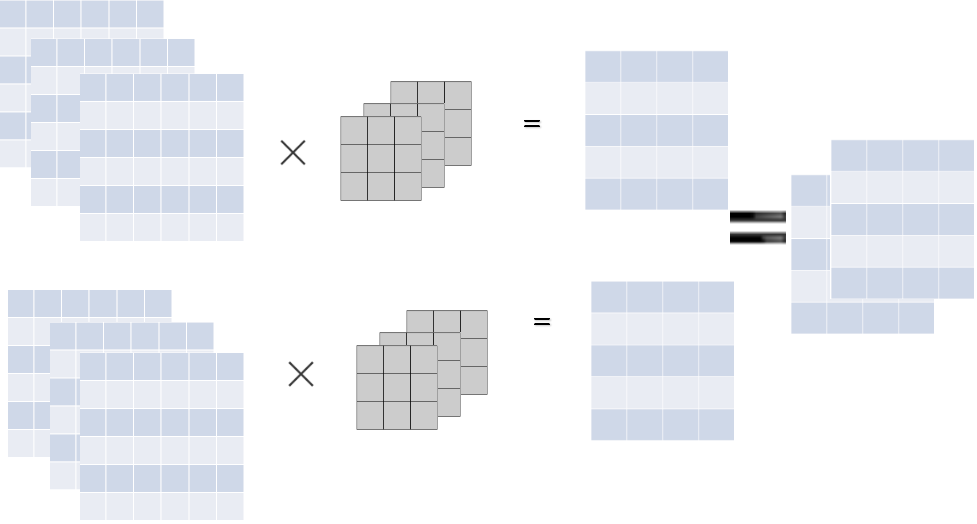
\includegraphics[width=.5\linewidth]{mainmatter/3-Methodology/images/cnn.png}
    \caption{Convolutional Neural Network}
    \label{fig:cnn}
  \end{figure}
  
  \iffalse
  \subsubsection{LSTM}
  As the \acrfull{rnn} often suffers from vanishing gradient problem~\footnote{Vanishing Gradient:During the training of RNN, the model vectors form a part of a loop and makes an unstable network.}, we use a \acrshort{lstm} Layer to learn the global pattern of the feature sets resulting after concatenation of different stacked layers outputs. The LSTM architecture can be seen in Figure ~\ref{fig:lstm}:
  \begin{figure} 
    [t]
    \centering
    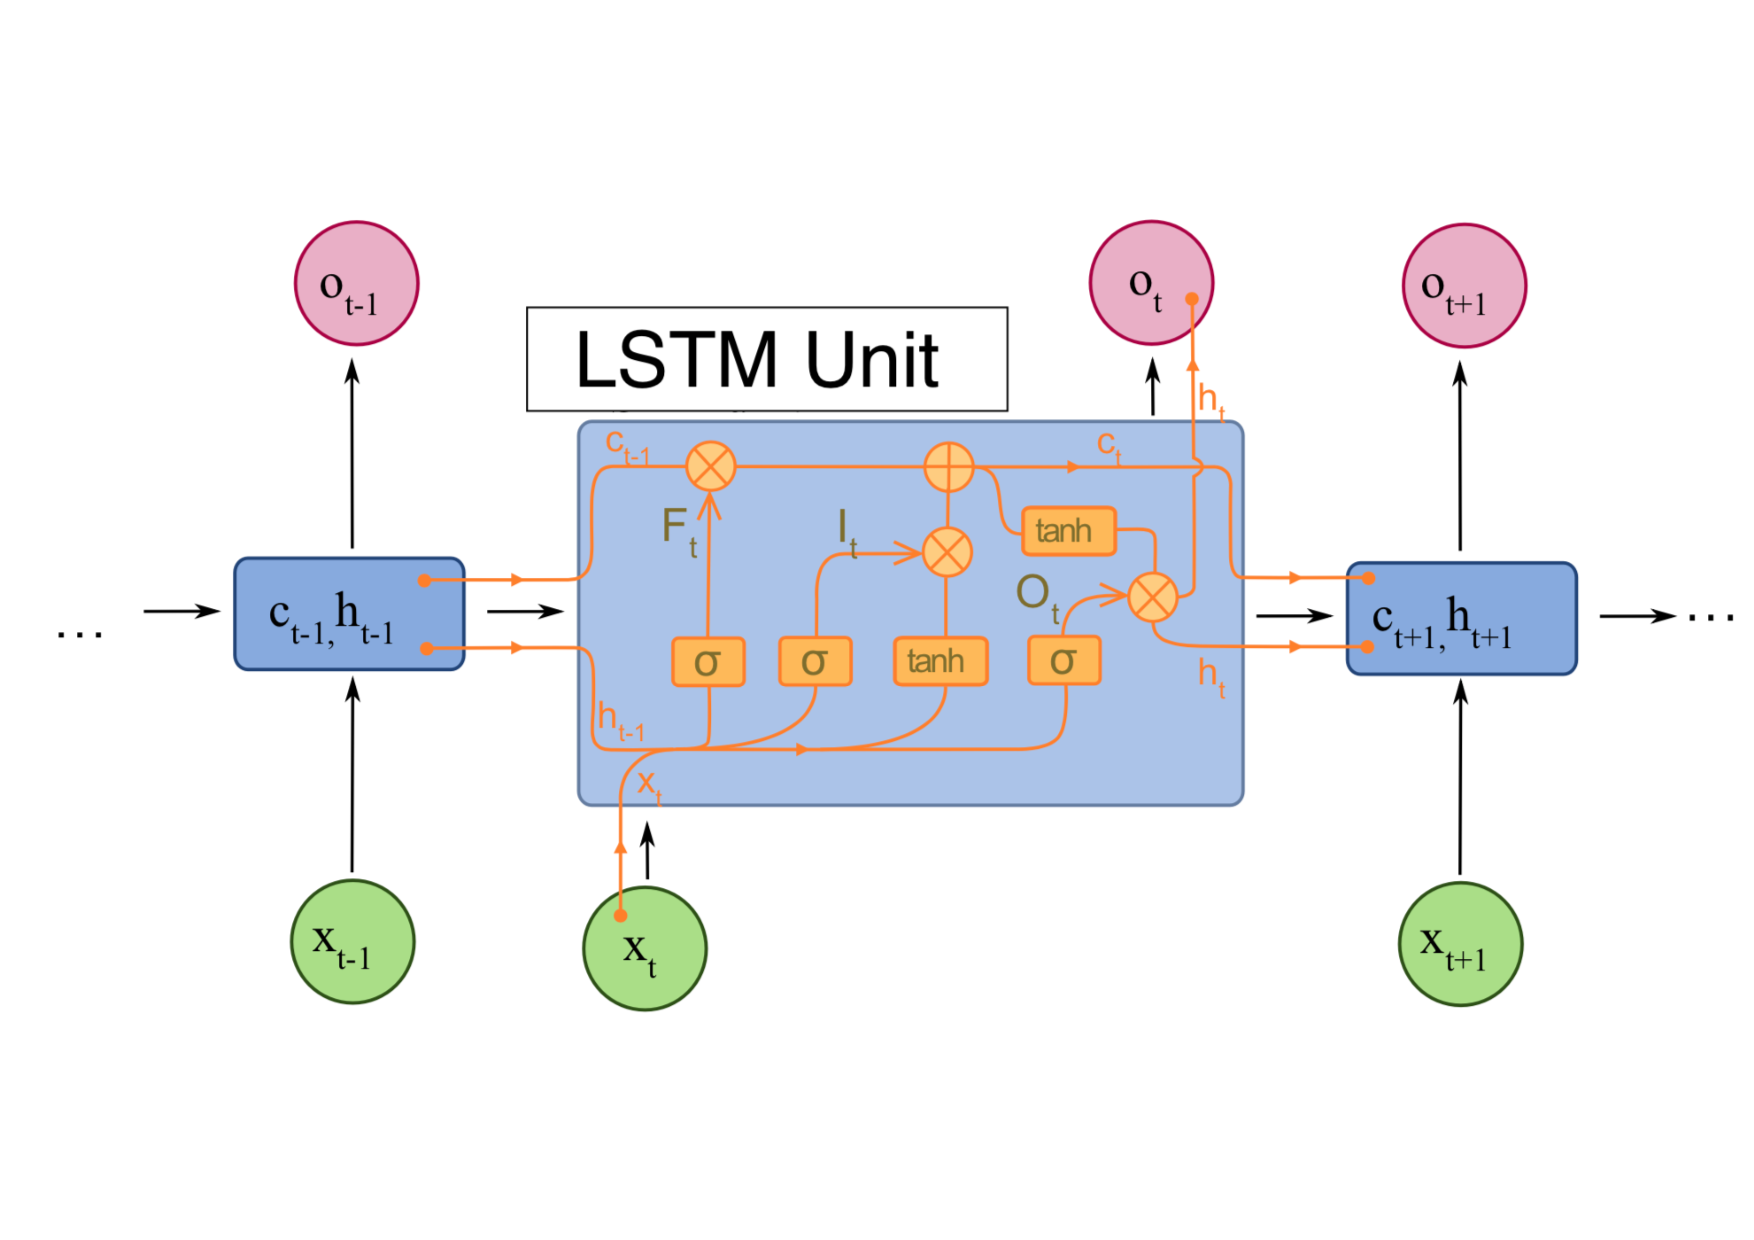
\includegraphics[width=1\linewidth]{mainmatter/3-Methodology/images/LSTM.pdf}
    \caption{Long Short Term Memory}
    \label{fig:lstm}
  \end{figure}
  In Figure~\ref{fig:lstm}, we can see that it contains a forget node, memory node and output node. These three nodes balance the information that needs to be removed, stored for future updates and necessarily fire the output node to make correct prediction.
  \fi